\documentclass{article}
\usepackage{geometry}
\usepackage{xcolor}
\usepackage{titlesec}
\usepackage{enumitem}
\usepackage{fancyhdr}
\usepackage{booktabs}
\usepackage{array}
\usepackage{graphicx}

% Define cola-inspired colors
\definecolor{colaRed}{RGB}{201, 37, 44}     % Deep red like Coca-Cola logo
\definecolor{colaBrown}{RGB}{58, 29, 20}    % Dark brown like cola liquid
\definecolor{colaCream}{RGB}{253, 246, 227} % Light cream for background
\definecolor{colaDark}{RGB}{45, 12, 7}      % Deep dark brown
\definecolor{violetPurple}{RGB}{138, 93, 150} % Violet flower color

% Page setup
\geometry{margin=1in}


% Header and footer setup
\pagestyle{fancy}
\fancyhf{}
\renewcommand{\headrulewidth}{0.4pt}
\renewcommand{\footrulewidth}{0.4pt}
\fancyhead[C]{\textcolor{violetPurple}{\textbf{Artisan Natural Fragrance Recipe}}}
\fancyfoot[C]{\textcolor{colaBrown}{\thepage}}

% Title format
\titleformat{\section}
  {\normalfont\Large\bfseries\color{colaRed}}
  {\thesection}{1em}{}

% Document begins
\begin{document}

\begin{center}
\textcolor{violetPurple}{\LARGE\textbf{Violet Cola Flower}}\\[0.5cm]
\textcolor{colaBrown}{\large\textit{A natural cola-inspired fragrance with floral depth and fruity sparkle}}\\[0.5cm]

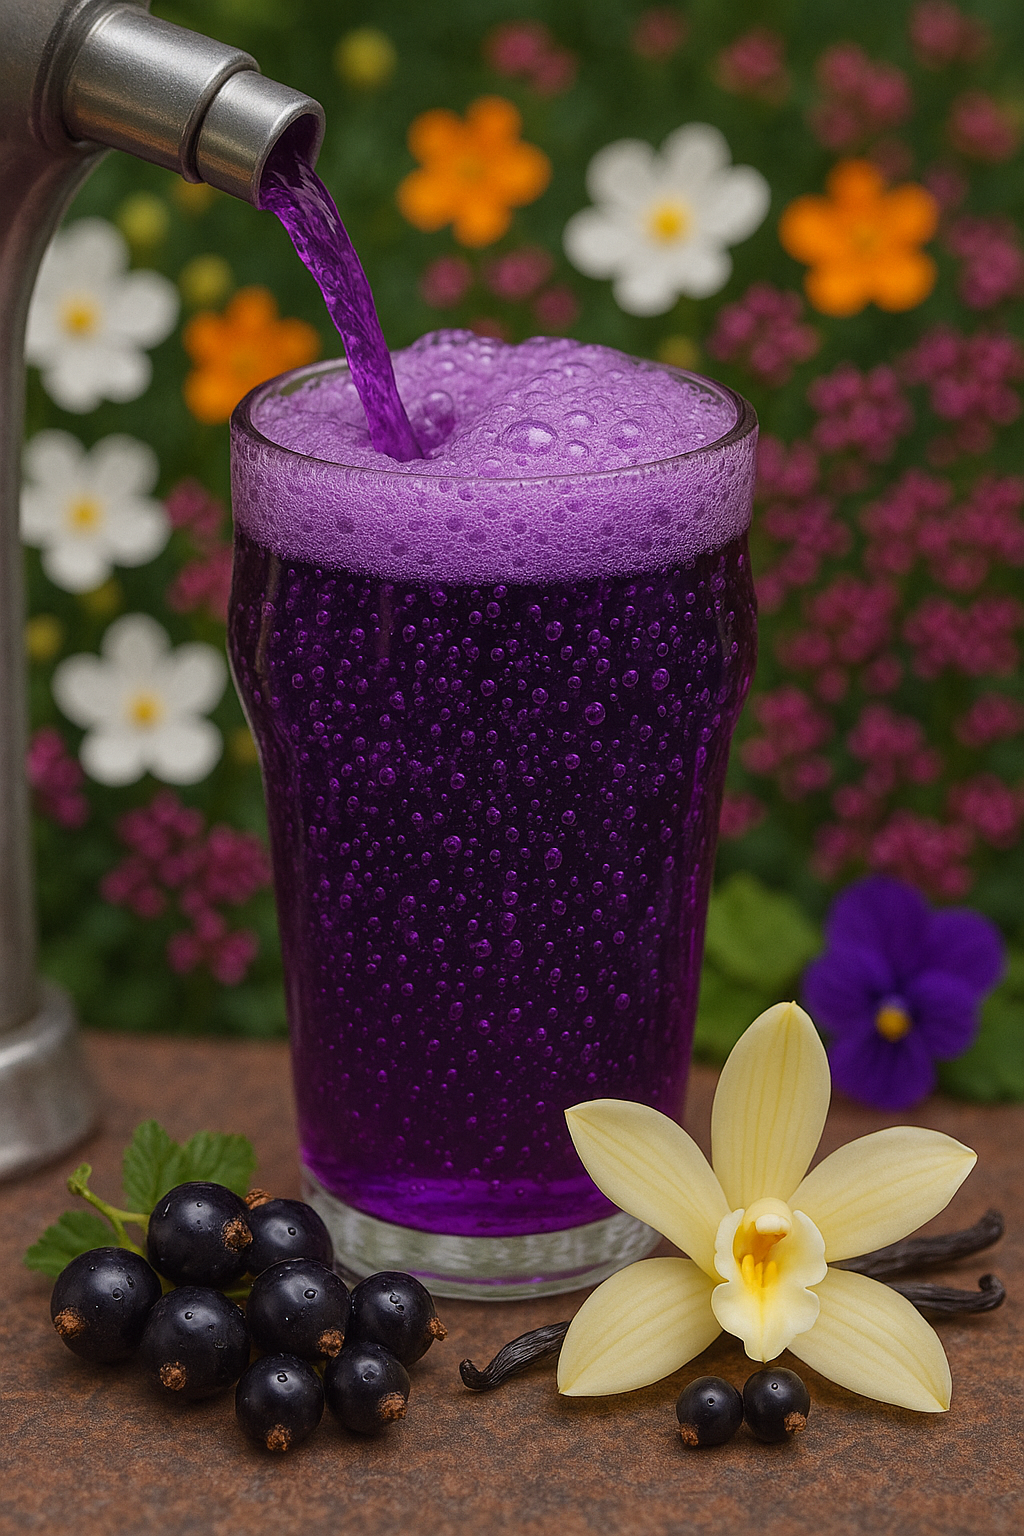
\includegraphics[width=0.7\textwidth]{violet_cola.png}\\[0.5cm]
\end{center}

\section*{Naturals-Only 1ml Fragrance Recipe}

\begin{center}
\begin{tabular}{p{6.5cm}r}
\toprule
\textcolor{colaRed}{\textbf{Ingredient}} & \textcolor{colaRed}{\textbf{Amount}} \\
\midrule
\multicolumn{2}{l}{\textcolor{violetPurple}{\textbf{Order of Addition (Bottom to Top):}}} \\
\midrule
IPM (Carrier) & 817 microliters \\
3\% Deer Musk Tincture & 33 microliters \\
10\% Boronia Absolute (in IPM) & 10 microliters \\
$\sim$10\% Black Currant Bud Absolute (in IPM) & 10 microliters \\
10\% Vanilla Absolute (in IPM) & 50 microliters \\
10\% Violet Leaf Absolute (in IPM) & 10 microliters \\
Nutmeg Absolute & 5 microliters \\
Neroli EO & 15 microliters \\
Pink Pepper EO (undiluted) & 10 microliters \\
Coriander EO & 10 microliters \\
Ceylon Cinnamon EO & 10 microliters \\
Lime EO & 30 microliters \\
Lemon EO & 30 microliters \\
Bergamot EO & 50 microliters \\
\bottomrule
\end{tabular}
\end{center}

\vspace{0.5cm}

\section*{Concentration Analysis}
\begin{itemize}[leftmargin=*]
  \item \textcolor{colaRed}{\textbf{Citrus Notes (11\%):}}
  \begin{itemize}
    \item Bergamot Essential Oil: 50 microliters (5\%)
    \item Lemon Essential Oil: 30 microliters (3\%)
    \item Lime Essential Oil: 30 microliters (3\%)
  \end{itemize}
  
  \item \textcolor{colaRed}{\textbf{Spice Elements (4\%):}}
  \begin{itemize}
    \item Ceylon Cinnamon Essential Oil: 10 microliters (1\%)
    \item Coriander Essential Oil: 10 microliters (1\%)
    \item Pink Pepper Essential Oil: 10 microliters (1\%)
    \item Neroli Essential Oil: 15 microliters (1.5\%)
    \item Nutmeg Absolute: 5 microliters (0.5\%)
  \end{itemize}
  
  \item \textcolor{violetPurple}{\textbf{Floral \& Fruit Notes (1.4\%):}}
  \begin{itemize}
    \item 10\% Violet Leaf Absolute: 10 microliters (0.1\% final)
    \item 10\% Vanilla Absolute: 50 microliters (0.5\% final)
    \item $\sim$10\% Black Currant Bud Absolute: 10 microliters ($\sim$0.116\% final)
    \item 10\% Boronia Absolute: 10 microliters (0.1\% final)
    \item 3\% Deer Musk Tincture: 33 microliters (0.1\% final)
  \end{itemize}
  
  \item \textcolor{colaBrown}{\textbf{Carrier:}}
  \begin{itemize}
    \item Isopropyl Myristate (IPM): 817 microliters (81.7\%)
  \end{itemize}
\end{itemize}

\section*{Expected Scent Profile}

% Caption for the image
\begin{center}
\textit{\small The vibrant purple color represents the violet and blackcurrant notes,\\
while the vanilla flower and blackcurrants illustrate key ingredients in this fragrance.}
\end{center}
\vspace{0.3cm}

\paragraph{\textcolor{colaRed}{\textbf{Top Notes (5-30 minutes):}}}
Bright citrus burst of bergamot, lemon, and lime with pink pepper's fruity-spicy sparkle and violet leaf's green fizz, mimicking the effervescence of freshly poured cola.

\paragraph{\textcolor{colaBrown}{\textbf{Heart Notes (30 min - 3 hours):}}}
Complex blend of spices (cinnamon, coriander, nutmeg), florals (neroli, boronia), and fruits (black currant). The black currant's tangy, sulfurous fruitiness adds cola-like depth, with variable intensity due to the $\sim$11.6\% dilution.

\paragraph{\textcolor{colaDark}{\textbf{Base Notes (3-6+ hours):}}}
Warm musky-sweet foundation from deer musk, vanilla, nutmeg, and traces of boronia, reminiscent of cola's lingering aftertaste.

\paragraph{\textcolor{violetPurple}{\textbf{Overall Performance:}}}
4-6 hours of wear with moderate projection, embodying a natural, artisanal character. This niche, natural cola interpretation features prominent citrus-spicy-floral notes, with black currant adding a variable tangy intensity.

\section*{Preparation Instructions}
\begin{enumerate}
  \item Begin with IPM carrier in a 1ml vial
  \item Add each ingredient in the specified order, using separate micropipette tips:
  \begin{itemize}
    \item Tip 1: IPM
    \item Tip 2: 3\% Deer Musk Tincture
    \item Tip 3: 10\% Boronia Absolute
    \item Tip 4: $\sim$10\% Black Currant Bud Absolute
    \item Tip 5: 10\% Vanilla Absolute
    \item Tip 6: 10\% Violet Leaf Absolute
    \item Tip 7: Nutmeg Absolute
    \item Tip 8: Neroli EO
    \item Tip 9: Pink Pepper EO
    \item Tip 10: Coriander EO
    \item Tip 11: Ceylon Cinnamon EO
    \item Tip 12: Lime EO
    \item Tip 13: Lemon EO
    \item Tip 14: Bergamot EO
  \end{itemize}
  \item Seal vial and roll gently to blend without introducing air bubbles
  \item Allow to rest 24-48 hours in a cool, dark place for notes to meld properly
  \item Test on skin, noting the prominence of black currant (adjust between 8-12 microliters if needed in future batches)
\end{enumerate}

\section*{Notes for Future Batches}
\begin{itemize}
  \item Black currant concentration may vary ($\sim$0.08-0.15\%). If too strong, reduce to 8 microliters; if too weak, increase to 12 microliters.
  \item For viscous ingredients, warming to 40-50°C for 10-15 minutes improves handling.
  \item When DPG arrives, consider remaking the 10\% dilutions for easier dissolution.
  \item Remaining black currant absolute (approximately 1.9g) should be stored in the fridge.
\end{itemize}

\vspace{1cm}
\begin{center}
\textcolor{violetPurple}{\rule{0.8\textwidth}{0.4pt}}
\end{center}

\begin{center}
\textit{\textcolor{colaDark}{A sophisticated all-natural interpretation of cola with vibrant citrus, delicate floral notes,\\
and tangy fruits balanced by warm spices and a musky foundation.}}
\end{center}

\end{document}
